\documentclass[a4paper,6pt,twocolumn,fleqn]{article}

\usepackage[margin=0.5in]{geometry}
\usepackage{nopageno}


\usepackage{amsmath,amssymb}
\usepackage{amsthm}
\usepackage{mathtools}

\usepackage{graphicx}
\usepackage{wrapfig}
\graphicspath{ {./} } %images path

\usepackage{algorithm2e}
\SetKwComment{Comment}{//}{}
\RestyleAlgo{ruled}
\SetAlgorithmName{Alg}{Alg}{List of Algorithms}
\SetAlCapFnt{\scriptsize}
\SetAlCapNameFnt{\scriptsize}
\SetAlFnt{\footnotesize}

\setcounter{secnumdepth}{0}

\begin{document}

\footnotesize

\section{Introduction}
\textbf{C.M. Bishop}: Machine Learning is concerned with the automatic discovery of regularities in data through the use of omputer algorithms and with the use of these regularities to take actions.\\
\textbf{K.P. Murpy}: The goal of Machine Learning is to develop methods that can automatically detect patterns in data, and then to use the uncovered patterns to predict future data or other outcomes of interest.\\
\textbf{Hal Daume III}: Machine Learning is about predicting the futre based on the past.\\
\textbf{T. Mitchell}: A computer program is said to learn from experience \(E\) with respect to some calss of tasks \(T\) and performance \(P\), if its performance at task in \(T\), as measured by \(P\), improves with experience \(E\).
\paragraph{Formally}
Machine Learning is the study of algorithms that improve their performance \(P\) at some task \(T\) with experience \(E\). A well-defined learning task is given by a triplet \(\langle T, P, E \rangle\).

\section{Data, Features, and Models}

\subsection{Learning process}
\begin{enumerate}
    \item Measuring devices --- sensors, cameras, databases;
    \item Preprocessing --- noise filtering, feature extraction, normalization;
    \item Dimensionality Reduction --- feature selection and/or projection;
    \item Model Learning --- classification, regression, clustering, description;
    \item Model Testing --- cross-validation, bootstrap;
\end{enumerate}
% subsection Learning process (end)
\subsection{Data}
\textbf{Data} are individual facts, statistics, or items of information, often numeric. Data are set of values of qualitative or quantitative variables about one or more persons or objects.
\begin{itemize}
    \item \textbf{Training data}: the part of data that we use to train our model. This is data that the model learns from.
    \item \textbf{Validation data}: the part of data that is used to do a frequent evaluation of the model, fit on the training dataset along with improving involved hyperparameters.
    \item \textbf{Test data} once the model is trained, test data provides an unbiased evaluation. After prediction, we evaluate our model by comparing it with the actual output present in the test data.
\end{itemize}
% subsection Data (end)
\subsection{Feature}
A \textbf{feature} is an individual measurable property or characteristic of a phenomenon. A \textbf{feature-vector} is an \(n\)-dimensional vector of numerical features that represent some object, and they are often combined with weights using a dot product in order to construct a linear predictor function.
% subsection Feature (end)
\subsection{Task} % (fold)
Tasks represent the type of prediction being made to solve a problem on some data. In general, it consists of functions assigning each input \(x \in X\) an output \(y \in Y\).
\begin{equation}
    f: X \to Y \qquad F_\text{task} \subset Y^X
\end{equation}
% subsection Task (end)
\subsection{Types of learning} % (fold)
\subsubsection{Supervised Learning} % (fold)
Build a mathematical model of a set of data that contains both the inputs and the desired outputs. Through iterative optimization of an objective function, supervised learning algorithms learn a function that can be used to predict the ouput associated
with new inputs.
\begin{itemize}
    \item \textbf{Classification}: problem of identifying which of a set of categories an observation belongs to.\\
    \textbf{Formally} given a training set \(T = \{(x_1, y_1), \ldots , (x_m,y_m)\}\), learn a function \(f\) to predict \(y\) given \(x\).
    \begin{itemize}
        \item \emph{Binary}: 
        \begin{equation}
            f: \mathbb R^1 \to \{1, 2, \ldots, k\}
        \end{equation}
        \item \emph{Multiclass}: 
        \begin{equation}
            f: \mathbb R^d \to \{1, 2, \ldots, k\}
        \end{equation}
    \end{itemize}
    \textbf{Task} find a function \(f \in Y^X\) assigning each input \(x \in X\) a discrete label
    \begin{equation}
        f(x) \in Y = \{c_1, c_2, \ldots, c_k\}
    \end{equation}
    \item \textbf{Regression}: set of statistical processes for estimating the relationships between a dependent variable and one or more independent variables.\\
    \textbf{Formally} given a training set \(T = \{(x_1, y_1), \ldots , (x_m,y_m)\}\), learn a function \(f\) to predict \(y\) given \(x\).
    \begin{equation}
        f: \mathbb R^d \to \mathbb R \qquad \text{ where } d=1
    \end{equation}
    \textbf{Task} find a function \(f(x) \in Y\) assigning each input a continuous label.
    \item \textbf{Ranking}: Data transformation in which numerical or ordinal values are replaced by their rank when the data are sorted.
\end{itemize}
% subsubsection Supervised Learning (end)
\subsubsection{Unsupervised Learning} % (fold)
Unsupervised learning algorithms take a set of data that contains only inputs, and find structure in the data, like grouping or clustering of data points.
\begin{itemize}
    \item \textbf{Clustering}: assignment of observations into subsets so that observation within the same cluster are similar accorting to one or more predesignated criteria.\\
    \textbf{Formally} given \(T = \{x_1, x_1, \ldots, x_m\}\) (without labels), the output is the hidden structure behind the \(x\)'s, that is the cluster.\\
    \textbf{Task} find a function \(f \in \mathbb N^X\) that assigns each input \(x \in X\) a cluster index \(f(x) \in \mathbb N\).
    \item \textbf{Anomaly detection}: identification of rare items, events or observations which raise suspicions by differing significantly from the majority of the data.
    \item \textbf{Dimensionality reduction}: process of reducing the number of random variables under consideration by obtaining a set of principal variables --- it is the process of reducing the feature set.\\
    \textbf{Task} find a function \(f \in Y^X\) mapping each input \(x \in X\) to a lower dimensional embedding \(f(x) \in Y\), where dim(\(Y\)) \(\ll\) dim(\(X\)) and \(Y = \mathbb R^2\).
    \item \textbf{Density estimation}: construction of an estimate, based on observed data, of an unobservable underlying probability density function.\\
    \textbf{Task} find a probability distribution \(f \in \Delta(x)\) that fits the data \(x \in X\).
\end{itemize}
% subsubsection Unsupervised Learning (end)
\subsubsection{Reinforcement Learning} % (fold)
Area of ML concerned with how intelligent agents ought to take actions in an environment in order to maximize the notion of cumulative reward. Reinforcement learning is the training of machine learning models to make a sequence of decisions. The agent learns to achieve a goal in an uncertain, potentially complex environment.
% subsubsection Reinforcement Learning (end)
% subsection Types of learning (end)

% section Data, Features, and Models (end)

\section{Models and Hypotesis space}
A \textbf{model} in machine learning is the output of a machine learning algorithm run on data. A model represents what was learned by a machine learning algorithm.

We assume that the set of all possible models is a subset \(H \subset F_\text{task}\), called \textbf{hypothesis space}.
\paragraph{Ideal target}
\begin{equation}
    f^* \in \arg \min_{f \in F_\text{task}} E(f; p_\text{data})
\end{equation}
\paragraph{Feasible target}
\begin{equation}
    f_H^* \in \arg \min_{f \in H} E(f; p_\text{data})
\end{equation}
\paragraph{Actual target}
\begin{equation}
    f_H^*(D_n) \in \arg \min_{f \in H} E(f; D_n)
\end{equation}
\subsection{Error function}
Typically in machine learning problems, we seek to minimize the error between the predicted value vs the actual value. The word error represents the penalty of failing to achieve the expected output. If the loss is calculated for a single training example, it is called or error function.

Typically, the generalization and training error function can be written in terms of a pointwise loss l(f; z) measuring the error incurred by f on the training example z.
\begin{equation}
    E(f; p_\text{data}) = E_{z \sim p_\text{data}} \left[l(f;z)\right]\\
    E(f;D_n) = \frac 1 n \sum_{i=1}^n l (f;z_i)
\end{equation}
\subsubsection{Overfitting}
Production of an analysis that corresponds too closely or exactly to a particular set of data, and may therefore fail to fit additional data or predict future observations.
% subsubsection Overfitting (end)
\subsubsection{Underfitting}
Occurs when a ML algorithm cannot adequately capture the underlying structure of the data. It occurs when the algorithm shows low variance but high bias.
% subsubsection Underfitting (end)
% subsection Error function (end)
\subsection{Generalization}
Generalization error cannot be computed for \(p_\text{data}\), so we use data sample, and we assume that the probability distribution is the same for the training set, for the validation set, and for the test set.

In order to improve the generalization well, there are number of approaches:
\begin{itemize}
    \item Avoid to obtain the minimum on training error;
    \item Reduce model capacity;
    \item Change the objective with a regularization term;
    \item Inject noise in the learning algorithm to smooht the data points;
    \item Stop the learning before the convergence.
\end{itemize}
\paragraph{Regularization}
Is the modification of the training error function with a term \(\Omega(f)\) that typically penalizes complex solutions.
\begin{equation}
    E_\text{reg} (f; D_n) = E (f; D_n) + \lambda_n \cdot \Omega(f)
\end{equation}
% subsection Generalization (end)
% section Models and Hypotesis space (end)

\section{\(k\)-Nearest Neighbors}
The training examples are vectors in a multidimensional feature space, each with a class
label. The training phase of the algorithm consists only of storing the feature vectors
and class labels of the training samples.

In the classification phase, \(k\) is a user-defined constant, and an unlabeled vector
is classified by assigning the label which is most frequent amongh the k training samples nearest to that query point.

\subsection{Distance}
\paragraph{Euclidean}
\begin{equation}
    D(a,b) = \sqrt{\sum_{d=1}^D \left(a_d - b_d\right)^2}
\end{equation}
\paragraph{Minkowski}
\begin{equation}
    D(a,b) = \left[\sum_{k=1}^p |a_k - b_k|^r\right]^{\frac 1 r}
\end{equation}
\paragraph{Cosine similarity}
\begin{equation}
    S_C (a,b) = \cos(\theta) = \frac {a \cdot b} {||a||\ ||b||}
\end{equation}
% subsection Distance (end)
\begin{algorithm}
    \caption{$k$-NN-classification(data, query, $k$, distance$_{fn}$)}
    neigDist $\gets [\ ]$\;
    \ForEach{$(index, example) \in data$}{
        dist $\gets$ distance$_{fn}($example.pop$()$, query$)$\;
        neigDist.append$(($dist$,$index$))$\;
    }
    sortedND $\gets$ sort$($neigDist$)$\;
    distList $\gets$ sortedND$[k]$\;
    labels $\gets [$distList.index$]$\;
    \Return{distList.counter$($labels$)$.mostCommon$()$}
\end{algorithm}
\subsection{Choosing \(k\)}
The best choice of \(k\) depends upon the data; generally, larger values of \(k\) reduces effect of the noise on the classification, but make boundaries between classes less distinct. A good \(k\) can be selected by various heuristic techniques.

The accuracy of the \(k\)-NN algorithm can be severely degraded by the presence of noisy or irrelevant features, or if the feature scales are not consistent with their importance
% subsection Choosing \(k\) (end)
\subsection{Weighted \(k\)-NN} % (fold)
Give more weight to the points which are nearby and less weight to the points which are farther away. The \(i\)-th nearest neighbour is assigned a weight \(w_{n_i}\) with
\begin{equation}
    \sum_{i=1}^n w_{n_i} = 1
\end{equation}
The algorithm is the same, but in the end we use the distance-weighted voting, that use the following formula
\begin{equation}
    y' = \arg \max_v \sum_{(x_i,y_i) \in D_z} w_i \times 1(v=y_i)
\end{equation}
where \(v\) represents the class labels.
% subsection Weighted \(k\)-NN (end)
% section k-Nearest Neighbors (end)

\section{Linear Models}
Linear models generate a formula to create a best-fit line to predict unknown values.
\subsection{Bias} % (fold)
The bias of a model is how strong the model assumptions are.
\begin{itemize}
    \item Low bias: minimal assumptions (\(k\)-NN, decision tree),
    \item High bias: strong assumptions about the data.
\end{itemize}
A strong high bias assumption is \textbf{linear separability}: can separate classes by a hyperplane.
A linear model in \(n\)-dimensional space is defined by \(n+1\) weights. The hyperplane can be used for classification by simply looking at the sign of the equation:
\begin{equation}
    b + \sum_{i=1}^n w_f \cdot f_i
\end{equation}
% subsection Bias (end)
\subsection{Online Learning} % (fold)
Method in which data becomes available in a sequential order and is used to update the best predictor for future data at each step.
Predictive model can be updated instantly for any new data instances, thus are more efficient and scalable for large-scale ML tasks.
% subsection Online Learning (end)
\subsection{Perceptron} % (fold)
The perceptron is an algorithm for learning a binary classifier called threshold function, that maps its input \(x\) to a value \(f(x)\):
\begin{equation}
    f(x) = \begin{cases}
        1 \qquad \text{if } w \cdot x + b > 0,\\
        0 \qquad \text{otherwise}
    \end{cases}
\end{equation}
The value of \(f(x)\) is used to classify \(x\) as either positive or negative instance. Spatically, the bias alters the position of the decision boundary.

The perceptron algorithm does not terminate if the learning set is not linearly separable. In order to prevent infinite loop we can use a maximum number of iteration.

\begin{algorithm}[h!]
\caption{Perceptron learning}
\label{alg:perceptron}
\While{convergence not reached}{
    \ForEach{training example $f_i$, label}{
        prediction $\gets b + \sum_{i=1}^nw_if_i$\;
        \If{not correct}{
            \ForEach{$w_i$}{
                $w_i \gets w_i + f_i \cdot$ label\;
            }
            $b \gets b +$ label\;
        }
    }
    }
\end{algorithm}
The perceptron algorithm guarantees that find some line, but not a special line.
% subsection Perceptron (end)
% section Linear Models (end)

\section{Decision trees}
Non-parametric supervised learning algorithm. The concept is to select splits that decrease the impurity of classes distribution in the resulting subsets of intstances.

Decision tree takes an inptu \(x \in X\). Each non-terminal node \(N(\phi,t_L,t_R)\) holds a routing function \(\phi \in {L,R}^X\), a left child \(t_L\) and a right child \(t_R\), that will be routed on based on the value of \(\phi(x)\).

When you do a split, each of the created descendant nodes corresponds to the applicable subset of the training data set. Nodes that are not split further become leaves, each leaf node \(L(h)\) holds a predition function \(h \in F_\text{task}\).

Given a training set \(D_n = \{z_1, z_2, \ldots, z_n\}\), the set \(T\) of all the possible decision trees, find \(f_{t^*}\), that corresponds to the optimal tree, where
\begin{equation}
    t^* \in \arg \min_{t \in T} E(f_t; D_n)
\end{equation}
We assume
\begin{equation}
    E(f_t;D) = \frac 1 {|D|} \sum_{z \in D} l(f;z)
\end{equation}
where \(l(f;z)\) is the pair-wise loss.
\paragraph{Growing a leaf}
Given \(D = \{z_1, z_2, \ldots, z_n\}\), the optimal leaf predictor that minimizes the local error can be computed as
\begin{equation}
    h_D^* \in \arg \min_{h \in H_\text{leaf} E(h;D)}
\end{equation}
The optimal error value is called impurity measure, and tells us what is the probability of misclassifying an observation --- the lower the impurity, the better the split.
\paragraph{Growing a node}
Given the set of all the possible routing functions \(\Phi\), and the training samples \(D\)
\begin{equation}
    \Phi_D^* \in \arg \min_{\phi \in \Phi} I_\phi(D)
\end{equation}
The impurity \(I_\phi(D)\) is computed in terms of the impurity of the split data
\begin{equation}
    I_\phi(D) = \sum_{d \in \{L,R}\} \frac {|D_d^\phi|} {|D|} I(D_d^\phi)\\
    D_d^\phi = \{(x,y) \in D;\ \phi(x) = d\}
\end{equation}
\begin{equation}
    \text{Grow}(D) = \begin{cases}
        L(h^*_D) \text{if stopping criterion met}\\
        N(\phi_D^*, \text{Grow}(D_L^*), \text{Grow}(D_R^*)) \text{otherwise}
    \end{cases}
\end{equation}
\subsection{Impurity measures} % (fold)
The error function can have different loss function that can lead to completely different error functions.
\subsubsection{Classification} % (fold)
\paragraph{Classification error}
\begin{equation}
    I(D) = 1 - \max_{y \in Y} \frac {|D^y|} {|D|}
\end{equation}
\paragraph{Gini impurity}
\begin{equation}
    I(D) = 1 - \sum_{y \in Y} \left( \frac {|D^y|} {|D|} \right)^2
\end{equation}
\paragraph{Entropy}
\begin{equation}
    I(D) = - \sum_{y \in Y} \frac {|D^y|} {|D|} \log \left( \frac {|D^y|} {|D|} \right)
\end{equation}
% subsubsection Classification (end)
\subsubsection{Regression} % (fold)
\paragraph{Variance}
\begin{equation}
    I(D) = \frac 1 {|D|} \sum_{(x,y) \in D)} || x - \mu_D ||^2
\end{equation}
% subsubsection Regression (end)
% subsection Impurity measures (end)
\subsection{Split functions} % (fold)
\paragraph{Discrete nominal features}
\begin{equation}
    \phi(x) = \begin{cases}
        L \qquad \text{if } x \in K_L\\
        R \qquad \text{if } x \in K_R
    \end{cases}
\end{equation}
\paragraph{Ordinal features}
\begin{equation}
    \phi(x) = \begin{cases}
        L \qquad \text{if } x \leq r\\
        R \qquad \text{if } x > r
    \end{cases}
\end{equation}
\paragraph{Oblique}
\begin{equation}
    \phi(x) = \begin{cases}
        L \qquad \text{if } w^T \cdot x \leq r\\
        R \qquad \text{otherwise} 
    \end{cases}
\end{equation}
% subsection Split functions (end)
\subsection{Pruning} % (fold)
Data compression technique that reduces the size of decision trees by removing sections in the tree that are non-critical and redundant to classify instances. Remove the nodes that do not provide additional information.
% subsection Pruning (end)
\subsection{Random Forests} % (fold)
We inject randomness into the tree building to ensure each tree is different.

Split functions are optimized on randomly samples features. The final prediction of the forest is obtained by averaing the prediction of each tree in the ensemble \(Q = \{t_1, t_2, \ldots, t_T\}\)
\begin{equation}
    f_Q(x) = \frac 1 T \sum_{j=1}^T f_t(x)
\end{equation}
\begin{algorithm}
\caption{Random Forest Learning}
\label{alg:perceptron}
\ForEach{$b \gets 1$ to $B$}{
    Draw a boostrap sample $\vec Z^*$ of size $N$ from the training data\;
    Grow a random-forest tree $T_b$ to the bootstrapped data\;
    \ForEach{terminal node $\in$ $T_b$}{
        \Repeat{minimum node size $n_\text{min}$ is reached}{
            Select $m$ variables at random from the $p$ variables\;
            Pick the best variable/split-point among the $m$\;
            Split the node into two daughter nodes\;
        }
    }
}
\Return{Output the ensemble of trees $T_b$}
\end{algorithm}
% subsection Random Forests (end)
% section Decision trees (end)

\section{Multiclass Classification}
Problem of classifying instances into one of three or more classes.

It is easy to think of a binary classifier as a black box, which can be reused for solving more complex problems.

\(k\)-NN and decision tree algorithms can by nature handle multiclass classification. Perceptron algorithm need some changes to fit the multiclass problem.

\subsection{One vs All (OVA)} % (fold)
You train \(K\)-many binary classifiers \(f_1, f_2, \ldots, f_K\). Classifier \(f_i\) receives all examples labeled class \(i\) as positives and all other examples as negatives.
\begin{algorithm}
\caption{OneVersusAllTrain($D^\text{multiclass}$, $BinaryTrain$)}
\label{alg:ovatrain}
\For{$i \gets 1,...,K$}{
    $D^\text{bin} \gets$ relabel $D^\text{multiclass}$ so class $i$ is positive, and class $\neg i$ is negative\;
    $f_i \gets \text{BinaryTrain}(D^\text{bin})$\;
}
\Return{$f_1,...,f_K$}
\end{algorithm}
\begin{algorithm}
\caption{OneVersusAllTest($f_1,...,f_K$, $x$)}
\label{alg:ovatest}
$score \gets \langle 0,0,...,0 \rangle$\;
\For{$i \gets 1,...,K$}{
    $y \gets f_i(x)$\;
    $score_i \gets score_i + y$\;
}
\Return{$\arg \max_k\ score_k$}
\end{algorithm}
% subsection One vs All (OVA) (end)
\subsection{All vs All (AVA)} % (fold)
\(f_{ij}\) for \(1 \leq i < j \leq K\) is the classifier that pits class \(i\) againts class \(j\).
\begin{algorithm}
\caption{AllVersusAllTrain($D^\text{multiclass}$, $BinaryTrain$)}
\label{alg:avatrain}
$f_{ij} \gets \emptyset, \forall 1 \leq i < j \leq K$\;
\For{$i \gets 1,...,K-1$}{
    $D^\text{pos} \gets$ all $x \in D^\text{multiclass}$ labeled $i$\;
    \For{$j \gets i+1,...,K$}{
        $D^\text{neg} \gets$ all $x \in D^\text{pos}$ labeled $j$\;
        $D^\text{bin} \gets \{(x, +1) : x \in D^\text{pos}\} \cup \{(x, -1) : x \in D^\text{neg}\}$\;
        $f_{ij} \gets BinaryTrain(D^\text{bin})$\;
    }
}
\Return{all $f_{ij}$}
\end{algorithm}
\begin{algorithm}
\caption{AllVersusAllTest(all $f_{ij}$, $x$)}
\label{alg:avatest}
$score \gets \langle 0, 0, ..., 0 \rangle$\;
\For{$i \gets 1,...,K-1$}{
    \For{$j \gets i+1,...,K$}{
        $y \gets f_{ij}(x)$\;
        $score_i \gets score_i + y$\;
        $score_j \gets score_j - y$\;
    }
}
\Return{$\arg \max_k\ score_k$}
\end{algorithm}
% subsection All vs All (AVA) (end)

\subsection{Evaluation} % (fold)
\begin{itemize}
    \item \textbf{micro-average} calculates the metric from the aggregate contributions of all classes. This is used for unbalanced datasets.
    \item \textbf{macro-average} calculates the metric autonomously for each class to calculate the average;
\end{itemize}
\subsubsection{Confusion matrix} % (fold)
\begin{figure}[h]
    \vspace{-10pt}
	\begin{center}
		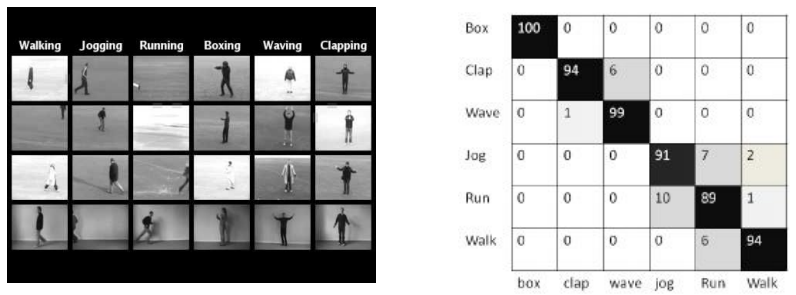
\includegraphics[width=0.45\textwidth]{036}
	\end{center}
    \vspace{-20pt}
\end{figure}
Shows the combination of the actual and predicted classes. The rows represent the predicted class and the columns represent the instances of the actual class.
% subsubsection Confusion matrix (end)
% subsection Evaluation (end)
% section Multiclass Classification (end)

\section{Gradient Descent}
First-order iterative optimization algorithm for finding a local minimum of a differentiable function.

\subsection{Optimization framework for linear models} % (fold)
In the case that your training data isn't linearly separable, you want to find the hyperplane that makes the fewest errors on the training data.
\begin{equation}
    \min_{w,b} \sum_n 1 \left[y_n (\vec w \cdot \vec x + b) > 0\right]
\end{equation}
If the optimum is zero, then the perceptron will efficiently find parameters for this model.
% subsection Optimization framework for linear models (end)
\subsection{Convex Surrogate Loss Functions} % (fold)
Convex functions are easy to minimize. We want to approximate zero/one loss with a convex function, called \textbf{surrogate loss} --- it will be the uppor bound on the true loss function.
\begin{align}
    \textbf{Zero/one: } &l^{(0/1)}(y, \hat y) = 1 [y \hat y \leq 0] \\
    \textbf{Hinge: } &l^{(\text{hin})}(y, \hat y) = \max \{0, 1 - y \hat y\} \\
    \textbf{Logistic: } &l^{(\text{log})}(y, \hat y) = \frac 1 {\log 2} \log (1 + \exp [-y \hat y]) \\
    \textbf{Exponential: } &l^{(\text{exp})}(y, \hat y) =  \exp [-y \hat y]\\
    \textbf{Squared: } &l^{(\text{hin})}(y, \hat y) = (y - \hat y)^2 \\
\end{align}
% subsection Convex Surrogate Loss Functions (end)
\subsection{Gradients} % (fold)
Multidimensional generalization of a derivative. The radient of \(f\) is just the vector consisting of the derivative \(f\) with respect to each of its input coordinates independently.
\begin{equation}
    \nabla_x f = \langle \frac {\delta f} {\delta x_1}, \frac {\delta f} {\delta x_2}, \ldots \frac {\delta f} {\delta x_D} \rangle
\end{equation}
% subsection Gradients (end)
\subsection{Optimization with gradient descent} % (fold)
At each step, it measures the gradient of the function that it is trying to optimize. It then takes a step in the direction of the gradient. The complete step is \(\vec x \gets \vec x + \eta g \).

\begin{algorithm}
    \caption{GradientDescent($F$, $K$, $\eta_1, ..., \eta_K$)}
    \label{alg:gradient_descent}
$\vec{z}^{(0)} = \langle 0,0,...,0 \rangle $\;
\For{$k \gets 1,...,K$}{
    $\vec{g}^{(k)} \gets \nabla_{\vec{z}} F |_{\vec{z}^{\,(k-1)}}$\;
    $\vec{z}^{(k)} \gets \vec{z}^{\,(k-1)} - \eta^{(k-1)} \vec{g}^{\,(k)}$\;
}
\Return{$\vec{z}^{\,(K)}$}
\end{algorithm}
% subsection Optimization with gradient descent (end)
\begin{align}
    \frac {\delta l} {\delta w_j} &= \frac \delta {\delta w_j} \sum_{i=1}^n \exp (-y_i (\vec w \cdot x_i + b)) \\
    & = \sum{i=1}^n -y_i \cdot x_{ij} \cdot \exp (-y_i (\vec w \cdot \vec x_i + b))
\end{align}
% section Gradient Descent (end)

\section{Regularization}
The goal is to ensure that the learned function does not overfit.

If you want the funcion to change slowly, you want to ensure that the weights stay small.

\begin{align}
    R^\text{(norm)} (\vec w, b) &= || \vec v || = \sqrt{\sum_d w_d^2}\\
    R^\text{(abs)} (\vec w, b) &= \sum_d |w_d|
\end{align}
\subsection{\(p\)-norm} % (fold)
This is a family of norms that have the same general flavor. \(||\vec w||_p\) denote the \(p\)-norm of \(\vec w\).
\begin{equation}
    ||\vec w||_p = R(\vec w, b) = \left[\sum_{w_j} |w_j|^p\right]^{\frac 1 p}
\end{equation}
\begin{figure}[h]
    \vspace{-10pt}
	\begin{center}
		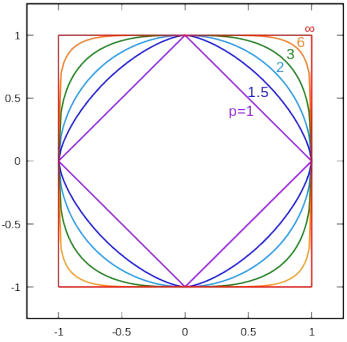
\includegraphics[width=0.25\textwidth]{040}
	\end{center}
    \vspace{-20pt}
\end{figure}
\subsubsection{L1 and L2 norms} % (fold)
L1 and L2 norms are common norms, and both push the weights to have smaller values close to zero.

Given the model
\begin{equation}
    \hat y = wx + b
\end{equation}

L1 regularizer gives a diamond, this means that one of the coordinates is different from zero, and the other is exactly zero.
\begin{align}
    L_1 &= (w x + b - y)^2 + \lambda |w|\\
    \frac {d|w|} {dw} &= \begin{cases}
        1 \qquad w > 0\\
        -1 \qquad w < 0
    \end{cases}
\end{align}

L2 regularizer gives a circle, that has no corner, it is very unlikely that the meet-point is on any of axes, but it is very close to zero.
\begin{equation}
    L_2 = (wx+b-y)^2 + \lambda w^2
\end{equation}
\paragraph{Gradient descent} 
\begin{equation}
    \min_{\vec w,b} \sum_{i=1}^n l(y \hat y) + \lambda R(\vec w)
\end{equation}
is convex as long as both the loss function and the regularizer are convex.

\begin{align}
    \text{L1: } & w_\text{new} = \begin{cases}
        w - \eta \cdot [2x (wx + b - y) + \lambda] \qquad w > 0\\
        w - \eta \cdot [2x (wx + b - y) - \lambda] \qquad w < 0
    \end{cases}\\
    \text{L2: } & w_\text{new} = w - \eta \cdot [2x (wx + b - y) + 2\lambda w]
\end{align}
% subsubsection L1 and L2 norms (end)
% subsection\(p\)-norm (end)
\subsection{Model-based ML} % (fold)
\begin{itemize}
    \item Pick a model
    \begin{equation}
        b + \sum_{j=1}^n w_j \cdot f_j = 0
    \end{equation}
    \item Pick the objective function 
    \begin{equation}
        \sum_{j=1}^n \exp (-y_i \cdot (\vec w x_i + b)) + \frac \lambda 2 ||\vec w||^2
    \end{equation}
    \item Develop a learning algorithm
    \begin{equation}
        \min_{\vec w,b} \sum_{j=1}^n \exp (-y_i \cdot (\vec w x_i + b)) + \frac \lambda 2 ||\vec w||^2
    \end{equation}
\end{itemize}
% subsection Model-based ML (end)
% section Regularization (end)
\section{SVM}
Optimization problem that attempts to find a separating hyperplane with as large margin as possible.

\textbf{Margin} of a data point: distance from the data point to a decision boundary.

\textbf{Margin classifier}: gives an associated sitance from the decision boundary for each example.

\textbf{Support vectors}: elemtns of the training set that would change the position of the dividing hyperplane if removed. For \(n\) dimension we have \(n+1\) suppor vectors.

The measure for the margin is defined by
\begin{figure}[h]
    \vspace{-10pt}
	\begin{center}
		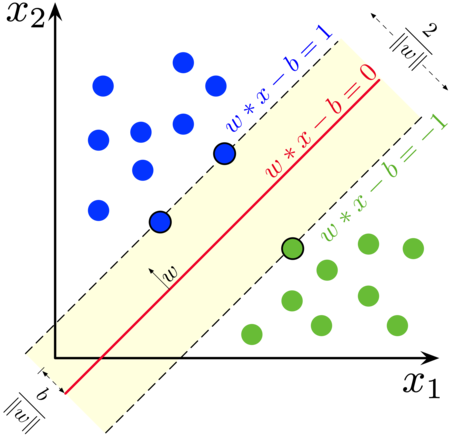
\includegraphics[width=0.30\textwidth]{042}
	\end{center}
    \vspace{-20pt}
\end{figure}
\begin{equation}
    \frac {\vec w \cdot \vec x_i + b} {||\vec w||} = \frac 1 {||\vec w||}
\end{equation}
Our goal is to \textbf{maximize the margin}
\begin{align}
    \max_{a,b} \text{margin}(\vec w, b) & = \max_{\vec w,b} \frac 1 {||\vec w||}\\
    & = \min_{\vec w, b} ||\vec w||
\end{align}
The support vetor machine problem is a version of a quadratic optimization problem
\begin{align}
    \min_{\vec w,b} || \vec w ||^2
    \text{subject to: } y_i \cdot (\vec w \cdot \vec x_i + b) \geq 1 \qquad \forall i
\end{align}

\subsection{Soft margin classification} % (fold)
If the training set \(D\) is not linearly separable, we allow the fat decision margin to make some mistake. We pay a cost for each misclassified example. To implement this we introduce \textbf{slack variables} \(\zeta_i\).

A non-zero value for \(\zeta_i\) allows \(\vec x_i\) to not meet the margin requirement at a cost proportional to the value of \(\zeta_i\).

The formulation of the SVM optimization problem with slack variable is:

Find \(\vec w\), \(b\) and \(\zeta_i>0\) such that:
\begin{align}
    &\min_{\vec w, b} ||\vec w||^2 + C \sum_i \zeta_i\\
    \text{subject to: } &y_i \cdot (\vec w \cdot \vec x_i + b) \geq 1 - \zeta_i \qquad \forall i, \zeta \geq 0
\end{align}
The sum of the \(\zeta_i\) gives an upper bound on the number of training errors.

\begin{align}
    \zeta_i & = \begin{cases}
        0 & \text{if } y_i \cdot (\vec w \cdot \vec x_i + b) \geq 1\\
        1 - y_i \cdot (\vec w \cdot \vec x_i + b) & \text{otherwise}
    \end{cases}\\
    & = \max\{0, 1 - y_i \cdot (\vec w \cdot \vec x_i + b)\}\\
    & = \max\{0, 1 - y \hat y\}\\
\end{align}
We can rewrite our optimization problem as
\begin{equation}
    \min_{\vec w,b} ||\vec w||^2 + C \sum_i \max\{0, 1 - y \hat y\}
\end{equation}
% subsection Soft margin classification (end)
\subsection{Non linearly separable data} % (fold)
\paragraph{Dual problem} Find \(\alpha_1, \alpha_2, \ldots, \alpha_n\) such that \(\sum_i \alpha_i - \frac 1 2 \sum_i \sum_j \alpha_i \alpha_j y_i y_j \vec x_i^T s_j\) is maximized and 
\begin{itemize}
    \item \(\sum_i \alpha_i y_i = 0\)
    \item \(\alpha_i \geq 0 \qquad \forall \alpha_i\)
\end{itemize}
Given a solution of the dual problem, the solution of the primal is
\begin{align}
    \vec w &= \sum_i \alpha_i y_i \vec x_i\\
    b &= y_k - \sum_i \alpha_i y_i \vec x_i^T \vec x_k \qquad \text{for any } \alpha_k > 0
\end{align}
The classifying function is 
\begin{equation}
    f(\vec x) = \sum_i \alpha_i y_i \vec x_i^T \vec x + b
\end{equation}
% subsection Non linearly separable data (end)
\subsection{Kernel trick} % (fold)
The linear classifier relies on inner product between vectors
\begin{equation}
    K(\vec x_i, \vec y_i) = \vec x_i^T \cdot \vec y_i
\end{equation}
If every datapoint is mapped into high-dimensional space via some transfomration \(\Phi: \vec x \to \phi(\vec x)\) the inner product becomes
\begin{equation}
    K(\vec x_i, \vec x_j) = \phi(\vec x_i)^T \cdot \phi(\vec x_j)
\end{equation}
A \textbf{kernel function} is a function that is equivalent to an inner product in some feature space.

\paragraph{Mercer's theorem} Every positive semidefinite symmetric function is a kernel. A positive semidefinite symmetric function corresponds to a positive emidefinite symmetric Gram matrix.

\begin{equation}
    K = 
    \begin{bmatrix}
        K(\vec{x}_1,\vec{x}_1) & K(\vec{x}_1,\vec{x}_2) & ... & K(\vec{x}_1,\vec{x}_n) \\
        K(\vec{x}_2,\vec{x}_1) & K(\vec{x}_2,\vec{x}_2) & ... & K(\vec{x}_2,\vec{x}_n) \\
        ... & ... & ... & ... \\
        K(\vec{x}_n,\vec{x}_1) & K(\vec{x}_n,\vec{x}_2) & ... & K(\vec{x}_n,\vec{x}_n) 
    \end{bmatrix}
\end{equation}

\paragraph{Kernels}
\begin{itemize}
    \item Linear: \(K(\vec{x}_i,\vec{x}_j) = \vec{x}_i^T\vec{x}_j\)
    \item Polynomial of power \(p\): \(K(\vec{x}_i,\vec{x}_j) = (1 + \vec{x}_i^T \vec{x}_j)^p\)
    \item Gaussian (radial-basis function): \(K(\vec{x}_i,\vec{x}_j) = e^{\frac {||\vec{x}_i - \vec{x}_j||^2} {2 \sigma^2}}\)
\end{itemize}

With the kernels, the dual problem formulation becomes
\begin{align*}
    &\max_\alpha \sum_i \alpha_i - \frac 1 2 \sum_i \sum_j \alpha_i \alpha_j y_i y_j K(\vec{x}_i, \vec{x}_j)\\
    \text{s.t. } &\sum_i \sum_j \alpha_i y_i = 0, \quad \alpha_i \geq 0, \quad \forall i
\end{align*}
And finally the solution is
\begin{equation}
    f(\vec{x}) = \sum_i \alpha_i y_i K(\vec{x}_i; \vec{x}) + b
\end{equation}
% subsection Kernel trick (end)
% section SVM (end)

\section{Ranking}
Produce a permutation of items in new, unseen lists in a similar way to rankings in the training data.

\paragraph{Multilabel classification} multiple labels may be assigned to each instance, each example has zero or more labels. Formally, is the problem of finding a model that maps inputs \(x\) to binary vectors \(y\).

\paragraph{Bipartite ranking} predict a binary response, for instance "is this document relevant or not?".

\subsection{Naive algorithm} % (fold)
\begin{algorithm}
    \caption{NaiveRankTrain(RankingData, BinaryTrain)}
    \label{alg:naive_rank_train}
    $D \gets [\ ]$\;
    \For{$n \gets 1$ to $N$}{
        \For{$i,j \gets 1$ to $M$ and $i \neq j$}{
            \eIf{$i$ is preferred to $j$ on query $n$}{
            $D \gets D.append(\vec{x}_{nij},+1)$\;
            }{
            \If{$j$ is preferred to $i$ on query $n$}{
                $D \gets D.append(\vec{x}_{nij},-1)$\;
            }
            }
    }
    }
\Return{BinaryTrain($D$)}
\end{algorithm}

\begin{algorithm}
    \caption{NaiveRankTest($f$, $\hat{x}$)}
    \label{alg:naive_rank_test}
$score \gets \langle 0, 0, ..., 0 \rangle$\;
\For{$i,j \gets 1$ to $M$ and $i \neq j$}{
    $y \gets f(\hat{x}_{ij})$\;
    $score_i \gets score_i + y$\;
    $score_j \gets score_j - y$\;
    }
    \Return{$score$.sort()}
\end{algorithm}

These algorithmswork well in case of bipartitte ranking problems.
% subsection Naive algorithm (end)
\subsection{Weighted binary classification} % (fold)
\paragraph{\(\omega\)-ranking} Given an input space \(\mathcal{X}\), an unknown distribution \(\mathcal{D}\) over \(\mathcal{X} \times \Sigma_M\), and a training set \(D\) sampled from \(\mathcal{D}\). We want to compute a function \(f : \mathcal{X} \to \Sigma_M\) minimizing:
\begin{equation}
    \mathbb{E}_{(\vec{x},\sigma) \sim \mathcal{D}} \left[ \sum_{u \neq v} [\sigma_u < \sigma_v] \cdot [\hat{\sigma}_v < \hat{\sigma}_u] \cdot \omega ( \sigma_u , \sigma_v ) \right]
\end{equation}
where \(\hat{\sigma} = f(\vec{x})\).

\begin{equation}
    \omega(i,j) = \begin{cases}
        1 &\text{if min}\{i,j\} \leq K \text{ and } i \neq j\\
        0 &\text{otherwise}\\
    \end{cases}
\end{equation}

\begin{algorithm}
    \caption{RankTrain($D^\text{rank}$, $\omega$, BinaryTrain)}
    \label{alg:rank_train}
    $D^\text{bin} \gets [\ ]$\;
    \For{$(\vec{x},\sigma) \in D^\text{rank}$}{
        \For{$u \neq v$}{
            $y \gets \text{sign}(\sigma_v - \sigma_u))$\;
            $w \gets \omega(\sigma_u - \sigma_v)$\;
            $D^\text{bin} \gets D^\text{bin} \oplus (y,w,\vec{x}_{uv})$\;
            }
            }
            \Return{BinaryTrain($D^\text{bin}$)}
        \end{algorithm}
        This algorithm is better than the naive algorithms because it make \(O(M \log_2 M)\) calls to \(f\) rather than \(O(M^2)\) class, and it achieves a better error bound.
        \begin{algorithm}
            \caption{RankTest($f$, $\hat{x}$, $obj$)}
            \label{alg:rank_test}
            \eIf{$obj$ contains 0 or 1 elements}{
    \Return{$obj$}
}{
    $p \gets$ randomly chosen object in $obj$\;
    $left \gets [\ ]$\;
    $right \gets [\ ]$\;
    \For{$u \in obj \setminus \{p\}$}{
        $\hat{y} \gets f(\vec{x}_{up})$\;
        \eIf{uniform random variable < $\hat{y}$}{
            $left \gets left \oplus u$\;
            }{
                $right \gets right \oplus u$\;
                }
                }
    $left \gets $ RankTest($f, \hat{x}, left$)\;
    $right \gets $ RankTest($f, \hat{x}, right$)\;
    }
    \Return{$left \oplus \langle p \rangle \oplus right$}
\end{algorithm}
% subsection Weighted binary classification (end)
% section Ranking (end)

\section{Neural Networks}
The idea of the multi-layer perceptron is to densely connect artifical neurons to realize compositions of non-linear functions. The information is propagated from the inputs to the outputs. No cycles between outputs and inputs (DAG). Compute one or more non-linear function. Computation is carried out by composition of some number of algebraic functions implemented by the connections, weights and biases of the hidden and output layers. Hidden layers compute intermediate representations.

\paragraph{Backpropagation}
Evaluates the gradient of the cost w.r.t. weights and biases.
\begin{itemize}
    \item Forward propagation: sum inputs, produce activations, feed-forward.
    \item Error estimation.
    \item Backpropagate the error signal and use it to update weights.
\end{itemize}
\subsection{Feedforward Networks} % (fold)
Information moves in only one direction, from the input nodes, through the hidden and to the output nodes.

The goal is to approximate some function \(f^* : \mathcal X \to \mathcal Y\).

\subsubsection{Training} % (fold)
The training examples specify directly what the output layer must do at each point \(\vec x\): it must produce a value that is close to \(y\). The other layers are not directly specified by the training data. The learning algorithm must decide how to use those layers to produce the desired output.

The nonlinearity of a NN causes most interesting loss functions to become non-convex. So NN are trained by iterative, gradient-based optimizers.

\paragraph{Cost function} The most common cost function is the \textbf{cross-entropy loss}
\begin{equation}
    \mathcal L_i = - \sum_k y_k \cdot \log(S(l_k)) = - \log(S(l))
\end{equation}

\paragraph{Activation function} Implemented inside the hidden units. The most popular is the \textbf{ReLU}, where \(h(x) = \max\{0,x\}\). It gives 1 if the gradient unit is active.

\textbf{Dying ReLU problem}: neurons can be pushed into states in which they become inactive for essentially all inputs. No gradients flow backward through the neuron, and so the neurom becomes stuck in an inactive state and \emph{dies}.

In order to mitigate these problems, there are some variants, for examples:
\begin{itemize}
    \item Leaky ReLU: \(y_i = a_i \cdot x_i\)
    \item Randomized Leaky ReLu: \(y_{ji} = a{ji} \cdot x_{ji}\)
\end{itemize}
Other activation function
\begin{itemize}
    \item \textbf{Sigmoid}: \(h(x) = \frac 1 {1 + e^{-x}}\)
    \item \textbf{Hyperbolic tangent}: \(h(x) = \frac {e^x - e^{-x}} {e^x + e^{-x}}\)
\end{itemize}
% subsubsection Training (end)
% subsection Feedforward Networks (end)
\subsection{Backpropagation} % (fold)
Algorithm for training FFNN. Computes the gradient of the loss function w.r.t. the weights of the network for a single input-output example, one layer at a time, iterating backword from the last layer to avoid redundant calculations in the chain rule.

\begin{enumerate}
    \item Feedforward propagation: accept input \(x\), pass through intermediate stages and optain output.
    \begin{equation}
        \hat{y} (\vec{x}; \vec{w}) = f \left( \sum_{j=1}^m w_j^{(2)} h \left( \sum_{i=1}^d w_{ij}^{(1)} x_i + w_{0j}^{(1)} \right) + w_0^{(2)} \right)
    \end{equation}
    \item Use the computed output to compute a scalar cost depending on the loss function.
    \begin{equation}
        L(X; \vec{w}) = \sum_{i=1}^N \frac 1 2 (y_i - \hat{y}(\vec{x}_i; \vec{w}))^2
    \end{equation}
    \item Backpropagation: allows information to flow backwards from cost to compute the gradient. The general unit activation in a multilayer network is 
    \begin{equation}
        z_t = h \left( \sum_j w_{jt} z_j \right)
    \end{equation}
    In forward propagation we calculate for each unit \(a_t = \sum_j w_{jt} z_j\).
    \begin{equation}
        \frac {\delta L} {\delta w_{jt}} = \frac{\delta L} {\delta a_t} \frac {\delta a_t} {\delta w_{jt}} = \frac {\delta L} {\delta a_t} z_j
    \end{equation}
    Key idea: it can be computed recursively starting from the final layer to the earlies layer.
\end{enumerate}
% subsection Backpropagation (end)
\subsection{Training} % (fold)
Adjust all the weights of the network \(\Theta\) such that a cost function is minimized
\begin{equation}
    \min_\Theta \sum_i L (y_i, f(x_i, \Theta))
\end{equation}
\subsubsection{Gradient Descent} % (fold)
\textbf{Batch Gradient Descent}

\begin{algorithm}
    \caption{BatchGradientDescent($k$)}
    \label{alg:batch_gradient_descent}
\KwData{Learning rate $\epsilon_k$}
\KwData{Initial parameter $\Theta$}
    \While{stopping criteria is not met}{
        $\hat{g} \gets \frac 1 N \nabla_\Theta \sum_i L\left( f(\vec{x}^{(i)}; \Theta), \vec{y}^{(i)} \right)$\;
        Apply Update: $\Theta \gets \Theta - \epsilon \hat{g}$\;
    }
\end{algorithm}

\textbf{Stochastic Gradient Descent}

\begin{algorithm}
    \caption{StochasticGradientDescent($k$)}
    \label{alg:stochastic_gradient_descent}
\KwData{Learning rate $\epsilon_k$}
\KwData{Initial parameter $\Theta$}
    \While{stopping criteria is not met}{
        Sample example $(\vec{x}^{(i)}, \vec{y}^{(i)})$ from training set\;
        $\hat{g} \gets \nabla_\Theta L\left( f(\vec{x}^{(i)}; \Theta), \vec{y}^{(i)} \right)$\;
        Apply Update: $\Theta \gets \Theta - \epsilon \hat{g}$\;
    }
\end{algorithm}

\textbf{Momentum}

\begin{algorithm}
    \caption{StochasticGradientDescent with Momentum}
    \label{alg:stochastic_gradient_descent_momentum}
\KwData{Learning rate $\epsilon_k$}
\KwData{Momentum parameter $\alpha$}
\KwData{Initial parameter $\Theta$}
\KwData{Learning velocity $\vec{v}$}
    \While{stopping criteria is not met}{
        Sample example $(\vec{x}^{(i)}, \vec{y}^{(i)})$ from training set\;
        $\hat{g} \gets \nabla_\Theta L\left( f(\vec{x}^{(i)}; \Theta), \vec{y}^{(i)} \right)$\;
        $\vec{v} \gets \alpha \vec{v} - \epsilon \hat{g}$\;
        Apply Update: $\Theta \gets \Theta - \epsilon \hat{g}$\;
    }
\end{algorithm}
% subsubsection Gradient Descent (end)
% subsection Training (end)
\subsection{Convolutional Neural Networks} % (fold)
The input is a tensof rwith a shape, given the number of inputs \(n\), the input height \(h\), the input width \(w\), and the input channels \(c\), the shape \(s\) is defined as
\begin{equation}
    s = n \cdot h \cdot w \cdot c
\end{equation}
After passing through a convolutional layer, the image becomes abstracted to a feature map, called activation map.
\subsubsection{Convolution} % (fold)
Mathematical operation on two functions \(f\) and \(g\) that produces a third function \(f \cdot g\) that expressed how the shape of one is modified by the other. A kernel matrix is applied to an image, and it works by determining the value of a central pixel by adding the weighted values of all its neighbors together.
\begin{align}
    S(i,j) &= (I \cdot K)(i,j)\\ 
    &= \sum_m \sum_n I(m,n) \cdot K(i-m,j-n)
\end{align}
The intuition is that the network will learn filters that activate when they see some specific type of feature at some spatial position in the input.
% subsubsection Convolution (end)
\subsubsection{Non-linearity} % (fold)
The result of the convolution is passed to an activation function
\begin{align}
    &y_{i,j} = f (a_{i,j})\\
    \text{e.g. } & f(a) = [a]_+\\
    & f(a) = \text{sigmoid}(a)
\end{align}
We are using non-linearity in order to have a final non-linear representation for our prediction model, and it doesn't affect the receptive field of the NN.
% subsubsection Non-linearity (end)
\subsubsection{Spatial Pooling} % (fold)
After the application of the non-linearity, spatial pooling is used to provide invariance to small traslation of the input.

It partitions the input image into a set of rectangles and, for each sub-region, outputs the maximum.

The pooling layer serves to progressively reduce the spatial size of the representation, to reduce the number of parameters, memory footprint and amount of computation in the network, and hence to control overfitting.
\begin{equation}
    x_{i,j} = \max_{|k| < \tau,\ |l| < \tau} y_{i-k,\ j-l}
\end{equation}
It is common to periodically insert pooling layer between successive convolutional layers.
% subsubsection Spatial Pooling (end)
% subsection Convolutional Neural Networks (end)
\subsection{Other Neural Networks} % (fold)
\subsubsection{Recurrent Neural Networks} % (fold)
Recurrent NN has been designed in problems in which we have multiple object as input and we want to predict multiple object as output. 

The particularity of the RNN is the recurrence formula, that is a function of certain parameters of the network that relates the input at time \(t\) ad the latent representation of the previous state with the latent representation of the current state:
\begin{equation}
    h_t = f_W(x_t, h_{t-1})
\end{equation}
% subsubsection Recurrent Neural Networks (end)
\subsubsection{Autoencoders} % (fold)
Can be considered as an unsupervised approach for learning a lower-dimensional feature representation from unlabeled data. There is a network that maps the original input data into low-dimensional latent representations.

The main idea is that the representation of the output \(z\) should be smaller than the input \(x\). The idea is to train the autoencoder so that features can be used to reconstruct original data.

Once we decided the architecture of the encoder and decoder, we need a loss function, and the loss function is a reconstruction function that minimizes the difference between the original data and the reconstructed version of the input data
\begin{equation}
    ||x - \hat x||^2
\end{equation}
\begin{figure}[h]
    \vspace{-10pt}
	\begin{center}
		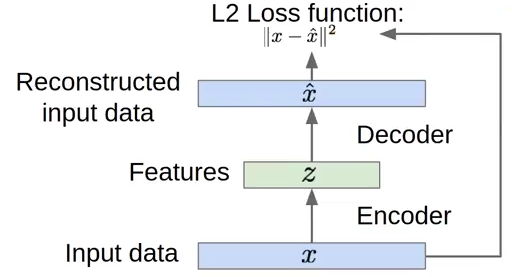
\includegraphics[width=0.30\textwidth]{063}
	\end{center}
    \vspace{-20pt}
\end{figure}
Once we have trained the autoencoder, we throw away the decoder, and we only take the latent representation \(z\) and we append the loss function \(\hat y\) and the encoder can be used to have a bettere initialization of a supervised model.
% subsubsection Autoencoders (end)
% subsection Other Neural Networks (end)
% section Neural Networks (end)

\section{Unsupervised Learning}
\subsection{Tasks} % (fold)
\subsubsection{Dimensionality Reduction} % (fold)
Transformation of data from high-dimensional space to low-dimensional space so that the low-dimensional space retain some meaningful properties of the original data.

Find a function \(f \in \mathcal Y^{\mathcal X}\) mapping each high-dimensional input \(x \in \mathcal X\) to a lower dimensional embedding \(f(x) \in \mathcal Y\) where \(dim(\mathcal Y) \ll dim(\mathcal X)\).
% subsubsection Dimensionality Reduction (end)
\subsubsection{Clustering} % (fold)
Grouping a set of objects in the same cluster that are more similar to each othern than to those in other groups.

Find a function \(f \in \mathbb N^{\mathcal X}\) that assigns each inptu \(x \in \mathcal X\) a cluster index \(f(x) \in \mathbb N\).
% subsubsection Clustering (end)
\subsubsection{Density Estimation} % (fold)
Construction of an estimate, based on observed data, of an unobservable underlying probability density function.

Find a probability distribution \(f \in \Delta(\mathcal X)\) that fits the data \(x \in \mathcal X\).
% subsubsection Density Estimation (end)
% subsection Tasks (end)
\subsection{Principal Component Analysis (PCA)} % (fold)
\textbf{Principal Component} sequence of \(p\) unit vectors, where the \(i\)-th vector is the direction of a line that best fits the data while being orthogonal to the first \(i-1\) vectors.

PCA is the process of computing the principal components and using them to perform a change of basis on the data, sometimes using only the first few PC.

We want to find the direction that explains the maximum variance of the data. Our second principal component is orthogonal to the first PC.

The way PCA allows us to do dimensionality reduction is by dropping the dimensions of least variance.

\paragraph{Variance along unit direction}
\begin{align}
    \mathbb E[t] & = \frac 1 n \sum_{i=1}^n t_i\\
    & = \bar{\vec x}^T \vec w - \vec c^T \vec w\\
    \mathbb Var[t] & = \frac 1 n \sum_{i=1}^n (t_i - \mathbb E[t])^2\\
    & = \vec w^T C \vec w
\end{align}
Where \(t_i = (\vec{x}_i - \vec{c})^T \vec{w}\), \(\bar{X} = [\bar{\vec{x}}_1, \bar{\vec{x}}_2, ..., \bar{\vec{x}}_n]\), and \(C = \left[ \frac 1 n \bar{X}\bar{X}^T \right]\) is the covariance matrix.

\subsubsection{Eigenvalue decomposition} % (fold)
Let \(A \in \mathbb{R}^{m \times m}\), symmetric. There exists \(U = \left[ \vec{u}_1, \vec{u}_2, ..., \vec{u}_m \right] \in \mathbb{R}^{m \times m} and \vec{\lambda} = (\lambda_1, \lambda_2, ..., \lambda_m)^T \in \mathbb{R}^{m}\) such that:
\begin{equation}
    A = U \Lambda U^T = \sum_{j=1}^m \lambda_j \vec{u}_j \vec{u}_j^T \qquad \text{and} \qquad U^T U = UU^T = I
\end{equation}
where \(U\) is the matrix of the eigenvectors, \(\Lambda\) is a square matrix with values all 0 except of the principal diagonal, that is composed by \(\lambda_1, \lambda_2, ..., \lambda_m\), \(I\) is the identity matrix, \(\vec{u}_j\) is an eigenvector and \(\lambda_j\) is the corresponding eigenvalue.

\paragraph{First PC}
\begin{equation}
    \vec{w}_1 \in \arg \max \left\{ \vec{w}^T C \vec{w} : \vec{w}^T \vec{w} = 1 \right\}
\end{equation}

\paragraph{Second PC}
\begin{equation}
    \vec{w}_2 \in \arg \max \left\{ \vec{w}^T C \vec{w} : \vec{w}^T \vec{w} = 1, \vec{w} \perp \vec{w}_1 \right\}
\end{equation}
% subsubsection Eigenvalue decomposition (end)

\subsubsection{PCA using Eigenvalue decomposition} % (fold)
\begin{algorithm}
    \caption{PCA using ED}
    \KwData{$X=\left[x_1,x_2,\ldots,n_n\right]$}
    $\bar X = X - \frac 1 n X 1_n 1_n^T$\;
    $C = \frac 1 n \bar X \bar X^T$\;
    $U$, $\lambda = $ eig$(C)$\;
    \Return{Principal components $W=U=[u_1,u_2,\ldots,u_m]$ and variances $\lambda = (\lambda_1, \lambda_2, \ldots, \lambda_m)$}
\end{algorithm}
% subsubsection PCA using Eigenvalue decomposition (end)
\subsubsection{Singular Value Decomposition} % (fold)
Let \(A \in \mathbb{R}^{m \times n}\). There exist \(U \in \mathbb{R}^{m \times k}, s \in \mathbb{R}^k\) with \(s_1 \geq s_2 \geq ... \geq s_k > 0\) and \(V \in \mathbb{R}^{n \times k}\) such that:
\begin{equation}
    A = USV^T \qquad \text{ and } \qquad U^TU = V^TV = I
\end{equation}
% subsubsection Singular Value Decomposition (end)

\subsubsection{PCA using SVD} % (fold)
\begin{algorithm}
    \caption{PCA using SVD}
    \KwData{$X=\left[x_1,x_2,\ldots,n_n\right]$}
    $\bar X = X - \frac 1 n X 1_n 1_n^T$\;
    $U$, $s$, $V = $ SVD$(\bar X)$\;
    \Return{Principal components $W=U=[u_1,u_2,\ldots,u_k]$ and variances $\lambda = \left( \frac {s_1^2} n, \frac {s_2^2} n, \ldots, \frac {s_k^2} n \right)$}
\end{algorithm}
% subsubsection PCA using SVD (end)
\subsubsection{Dimensionality Reduction with PCA} % (fold)
If we compute 
\begin{equation}
    T = \hat W^T \bar X \in \mathbb R^{k \times n}
\end{equation}
will induce a change of the coordinate system w.r.t. the \(k\) principal components in \(\hat W^T\), and this will reduce the dimension of the features to \(k\).
% subsubsection Dimensionality Reduction with PCA (end)
\paragraph{How Many PC?}
\begin{itemize}
    \item depends on the goal
    \item no means of validating it, unless supervised learning
    \item we can compute the cumulative proportion of expaired variance
    \begin{equation}
        \text{ED: } \frac {\sum_{j=1}^k \lambda_j} {\sum_{j=1}^m C_{jj}} \qquad \text{SVD: } \frac {\sum_{j=1}^k s_j^2} {\sum_{ij} \bar X_{ji}^2}
    \end{equation}
    \begin{itemize}
        \item allows to estimate the amount of information loss
    \end{itemize}
\end{itemize}
% subsection Principal Component Analysis (PCA) (end)
% section Unsupervised Learning (end)

\section{Clustering}
\subsection{\(k\)-means Clustering} % (fold)
Given data points \(X = [x_1, x_2, \ldots, x_n] \in \mathbb R^\{d \times n\}\) and \(k\) a fixed number of clusters. Our goal is to find a partition of data points into \(k\) sets \(\mathcal C_1, \mathcal C_2, \ldots, \mathcal C_k\) minimizing the variation \(V(\mathcal C_j)\) within eahc set:
\begin{equation}
    \min_{\mathcal C_1,\ldots,\mathcal C_k} \sum_{j=1}^k V(\mathcal C_j)\\
    V(\mathcal C_j) = \sum_{i \in \mathcal C_j} || \vec x_i - \vec \mu_j||^2
\end{equation}
where \(\mu_j\) is the centroid of \(\mathcal C_j\).

\begin{algorithm}
    \caption{$k$-means}
    Use some initialization strategy to get some initial cluster centroids $\mu_1,\ldots,\mu_k$\;
    \While{clusters change}{
        Assign each datapoint to the closest centroid forming new clusters\;
        $\mathcal C_j = \{i \in \{1,\ldots,n\} : j = \arg \min_l ||\vec x_i - \mathcal \mu_l\}$\;
        Compute the cluster centroids $\mu_1,\ldots,\mu_k$\;
    }
\end{algorithm}
\paragraph{Properties}
\begin{itemize}
    \item guarantees to converge,
    \item it is not guaranteed to find the global minimum, but a local one
    \item centroids selection plays an important role with the result.
\end{itemize}
\paragraph{Centroids selection}
\begin{itemize}
    \item random points (not examples) in the space;
    \item random examples;
    \item points least similar to any existing center;
    \item try multiple starting points;
    \item initialize with the results of another clustering method;
\end{itemize}
% subsection \(k\)-means Clustering (end)
\subsection{Issues for Clustering}
\begin{itemize}
    \item how to represent data points?
    \item the way we choose to measure the distance;
    \item does the problem necessitate of flat or hierarchical clustering?
    \item how to define the number of cluster.
\end{itemize}
\paragraph{Types of clustering}
\begin{itemize}
    \item \textbf{Flat algorithms}: start with a random partitioning and refines it iteratively.
    \item \textbf{Hierarchical algorithms}: bottom-up agglomerative or top-dow divisive.
    \item \textbf{Hard clustering}: each example belongs to exactly one cluster.
    \item \textbf{Soft clustering}: an example can belong to more than one cluster.
\end{itemize}
% subsection Issues for Clustering (end)
\subsection{EM Clustering} % (fold)
Assumes that data came from mixture of gaussians. Assigns data to cluster with a certain probability. Follows an iterative scheme as \(k\)-means, iterates between assigning points and recalculating cluter centers.
\begin{algorithm}
    \caption{EM Clustering}
Initialize clusters\;
\While{clusters does not change}{
    Calculate \(p(\Theta_c | x)\) the probability of each point belonging to each cluster\;
    Recalculate the new cluster parameters \(\Theta_c\), the maximum likelihood cluster centers given the current soft clustering\;
}
\end{algorithm}
EM stands for
\begin{itemize}
    \item \textbf{Expectation}: given the current model, figure out the expected probabilities of the daa points to each cluster \(p(\Theta_c|x)\).
    \item \textbf{Maximization}: given the probabilistic assignment of all the points, estimate a new model \(\Theta_c\).
\end{itemize}
% subsection EM Clustering (end)
\subsection{Other Clustering Algorithms} % (fold)
\paragraph{Spectral clustering}
We form a matrix that indicate the similarity of each data point w.r.t. each other. In can be represented in terms of graphs, where each edge indicates the similarity between two points.

We can create a fully connected graph, or a \(k\)-nearest neighbor graph. We can create a graph with some notion of similarity among nodes, gaussian kernel:
\begin{equation}
    W(i,j) = \exp \left\{ \frac {-|x_i - x_j|^2} {\sigma^2} \right\}
\end{equation}
\(Cut(A,B)\) is the sum of the weights of the set of edges that connect two groups. An intuitive goal is to find the partition that minimizes the cut.
\paragraph{Hierarchical clustering}
Produce a set of nested clusters organized as a hierarchical tree (\textbf{dendogram}).
\paragraph{Agglomerative clustering} First merge very similar instances and then incrementally build larger clusters out of smaller clusters.
\begin{algorithm}
    \caption{Agglomerative clustering}
    Each instance in its own cluster\;
    \Repeat{until there is only one cluster}{
        Pick the two closest clusters\;
        Merge them into a new cluster\;
    }
    \Return{Family of clusterings represented by a dendogram}
\end{algorithm}
% subsection Other Clustering Algorithms (end)
% section Clustering (end)

\section{Deep generative models}
\begin{itemize}
    \item \textbf{Generative}: statistical models of the data distribution \(p_X\) or \(p_{XY}\) depending on the availability of target data.
    \item \textbf{Discriminative}: statistical models of the conditional distribution \(p_{X|Y}\) of the target given the input. 
\end{itemize}
A discriminative model can be constructed from a generative model via the Bayes rule, but not vice versa
\begin{equation}
    p_{X|Y} (y,x) = \frac {p_{XY}(x,y)} {\sum_{\hat y} p_{XY} (x, \hat y)}
\end{equation}
\subsection{Density Estimation} % (fold)
We want to find the probability distribution \(f \in \Delta (\mathcal Z)\) that fits teh data \(z \in \mathcal Z\), where \(z\) is sampled from unknown data distribution \(p_\text{data} \in \Delta (\mathcal Z)\), and \(\mathcal Z = \mathcal X \times \mathcal Y\).

Objectives:
\begin{itemize}
    \item define an hypothesis space \(\mathcal H \subset \Delta(\mathcal Z)\) of models that can represent probability distributions
    \item define a divergence measure \(d \in \mathbb R^{\Delta (\mathcal Z) \times \Delta (\mathcal Z)}\) between probability distributions \(\Delta (\mathcal Z)\)
    \item find an hypothesis \(q^* \in \mathcal H\) that best fits the data distributed according to \(p_\text{data}\).
    \begin{equation}
        q^* \in \arg \min_{q \in \mathcal H} d(p_\text{data}, q)
    \end{equation}
\end{itemize}
% subsection Density Estimation} (end)
\subsection{Variational AutoEncoder (VAE)} % (fold)
Compressing high-dimensional data into a lower dimensional representation.
\textbf{Encoder}: maps input data \(x\) to a compressed representation \(\omega\) that preserves meaningful factors of variations in the data.

Encoder is trained by leveraging a decoder mapping the representation \(\omega\) back to the input domain yielding \(\hat x\) (\textbf{reconstruction}).

The objective is to minimize the divergence between input \(x\) and its reconstruction \(\hat x\).

After training the decoder is not needed anymore, since it was only functional to estimate the encoder.

\begin{figure}[h!]
    \vspace{-10pt}
	\begin{center}
    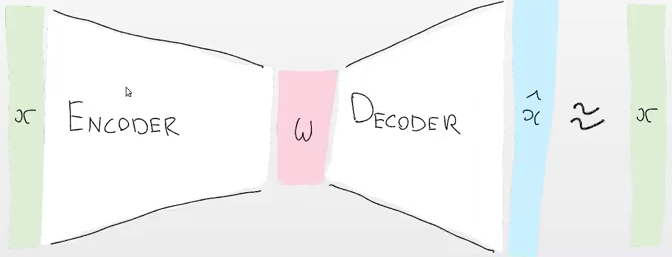
\includegraphics[width=.4\textwidth]{083}
    \end{center}
    \vspace{-20pt}
\end{figure}

\begin{figure}[h!]
    \vspace{-10pt}
	\begin{center}
    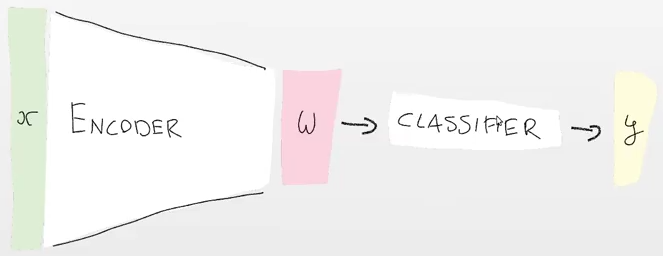
\includegraphics[width=.4\textwidth]{084}
    \end{center}
    \vspace{-20pt}
\end{figure}

\subsubsection{In generative models} % (fold)
Given a latent space \(\Omega\) with a prior distribution \(p(\omega)\), and an input space \(\mathcal X\) with a data distribution \(p_\text{data}(x)\). We want a decoder that produce a mapping from the latent space to the input space where the regions of low probability of the latent input space correspond to the region of the low probability of the latent space, and the same thing with the region of high probability.
\begin{align}
    & q_\theta (x) = \mathcal E_{\omega \sim p_\omega}[ q_\theta (x | \theta) ]\\
    & \theta^* \in \arg \min_{\theta in \Theta} d(q_\theta, p_\text{data})
\end{align}
\paragraph{Kullback-Leibler divergence} (distance)
\begin{equation}
    d_{KL} (p,q) = \mathbb E{x \sim p} \left[\log \frac {p(x)} q(x) \right]
\end{equation}
but we end up in an intractable problem.
% subsubsection In generative models (end)
\subsubsection{Variational Upper Bound} % (fold)
Let \(q_\psi (\omega | x) \in \Delta(\Omega)\), where \(\psi\) defines other parameters, denote an encoding probability distribution:
\begin{equation}
    \log \mathbb{E}_{\omega \sim p_\omega} \left[ q_\theta (x | \omega) \right] = \underbrace{ \mathbb{E}_{\omega \sim p_\psi(\cdot | x)} \left[ \log q_\theta (x | \omega) \right] }_\text{Reconstruction} - \underbrace{ d_{KL}(q_\psi(\cdot | x), p_\omega) }_\text{Regularizer}
\end{equation}
Now we can define a variational bound:
\begin{equation}
    d_{KL} (p_\text{data}, q_\theta) \leq \mathbb{E}_{x \sim p_\text{data}} \left[
        - \mathbb{E}_{\omega \sim p_\psi(\cdot | x)} [\log q_\theta (x | \omega)] + d_{KL}(q_\psi(\cdot | x), p_\omega)
    \right] + const
\end{equation}
The reconstruction is still intractable to compute, but is easy to get unbiased estimates of gradients with respect to \(\theta\) and \(\psi\). The regularizer might have closed-form solution, e.g. using gaussian distributions.
% subsubsection Variational Upper Bound (end)
\paragraph{Issues with VAE}
\begin{itemize}
    \item generator tends to produce blurry data;
    \item underfitting, in particular the balance between the regularization and the reconstruction terms must be managed carfully.
\end{itemize}
% subsection Variational AutoEncoder (VAE) (end)
\subsection{Generative Adversarial Networks (GAN)} % (fold)
The idea is to have an implicit density model, so not requiring to estimate \(q_\theta(x)\).

Enable the possibility of estimating implicit density. We assume to have a prior density \(p_\omega \in \Delta(\Omega)\) and a generator (decoder) \(g_\theta \in \mathcal X^\Omega\) that generates data points in \(\mathcal X\) given a random element from \(\Omega\).
\begin{equation}
    q_\theta (x) = \mathbb E_{\omega \sim p_\omega} \delta [ g_\theta (\omega) - x ]
\end{equation}
where \(\delta\) is the Dirac delta function.

\paragraph{Objective}
Find \(\theta^*\) such that \(q_{\theta^*}\) best fits the data distribution \(p_\text{data}\).

\begin{figure}[h!]
    \centering
    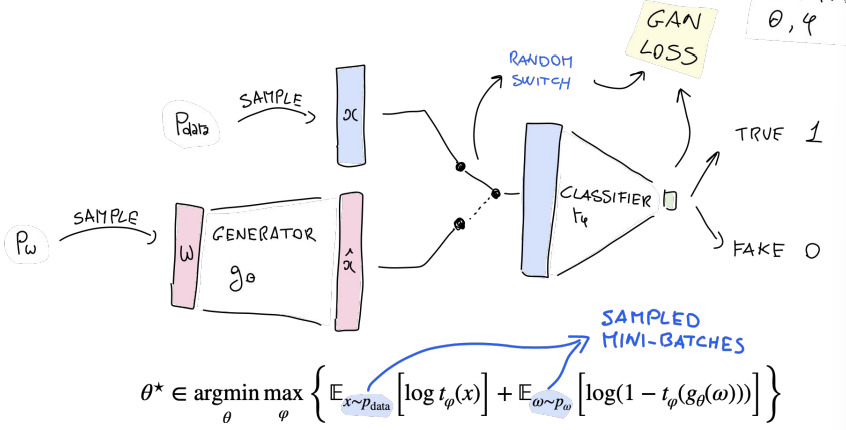
\includegraphics[width=.4\textwidth]{101}
    \label{fig:101}
\end{figure}

\paragraph{Issues}
\begin{itemize}
    \item training stability: since we have the alternation between the generator and the discriminator, the parameters of the network may oscillate and never converge
    \item mode collapse: the generator might learn to perfectly generate few examples from the training set, but not cover all the variability that is in the training set
    \item vanishing gradient: if the discriminator is successful, then it will have a little gradient to learn, so it leaves the generator with little gradient to learn from.
\end{itemize}
% subsection Generative Adversarial Networks (GAN) (end)
% section Deep generative models (end)

\section{Reinforcement Learning}
The problems involve an \textbf{agent} interacting with an \textbf{environment}, which provides numeric \textbf{rewards} signals.

The goal is to learn a \textbf{policy} to maximize the expected reward over time.
\textbf{policy}: mapping from states to actions.

\begin{figure}[h!]
    \centering
    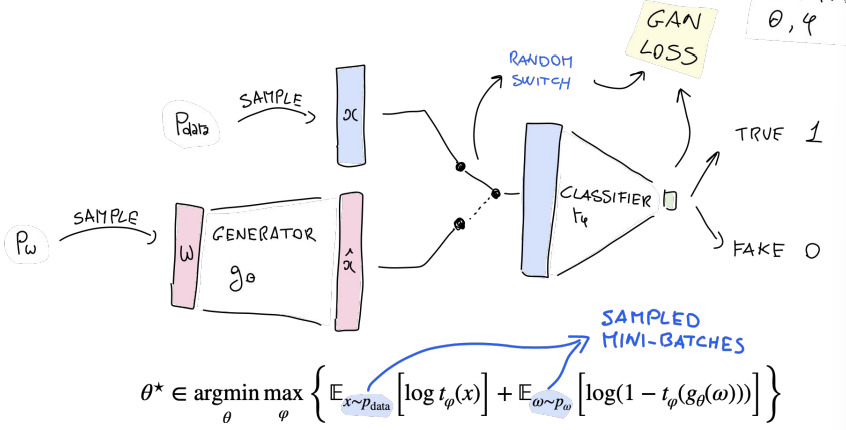
\includegraphics[width=.4\textwidth]{101}
    \label{fig:090}
\end{figure}

\subsection{Markov Decision Procedd} % (fold)
Framework used to help to make decisions on a stochastic environment. Goal si to find a policy, which is a map that gives us all optimal actions on each state in our environment.

Probability that the process moves into its new state \(s'\) is influenced by the chosen action. It is given by the state transaction function \(P_a(s,s')\). \(s'\) depends on \(s\) and the decision maker's action \(a\).

\textbf{MDP}: 5-tuple \((\mathcal S, \mathcal A, \mathcal R, P, \gamma)\)
\begin{itemize}
    \item \(\mathcal S\) is the state space.
    \item \(\mathcal A\) is the action space.
    \item \(\mathcal R_a(s,s')\) is the reward received after transitioning from state \(s\) to \(s'\).
    \item \(P_a(s,s')\) is the probability that action \(a\) in state \(s\) at time \(t\) will lead to state \(s'\) at time \(t+1\).
    \item \(\gamma\) discount factor.
\end{itemize}
A policy function \(\pi\) is a mapping from state space \(\mathcal S\) to an action space \(\mathcal A\).

\paragraph{Loop}
\begin{itemize}
    \item Agent selects action \(a_t\);
    \item Environment samples reward \(r_t \sim \mathcal R( \cdot | s_t, a_t)\);
    \item Environment samples next state \(s_{t+1} \sim P( \cdot | s_t, a_t)\);
    \item Agent receives reward \(r_t\) and next state \(s_{t+1}\).
\end{itemize}
\paragraph{Objective}
find a good policy for the decision maker: a function \(\pi\) that specifies the action \(\pi(s)\) that the decision maker will choose when in state \(s\).

Choose a policy \(\pi\) that will maximize some cumulative function of the random rewards (called optimal policy \(\pi^*\)).

\paragraph{Cumulative reward}
\begin{equation}
    r(s_0) = \gamma r(s_1) + \ldots = \sum_{t \geq 0} \gamma^t r(s_t) \qquad 0 < \gamma \leq 1
\end{equation}
% subsection Markov Decision Procedd (end)

\subsection{Reinforcement vs Supervised} % (fold)
Supervised:
\begin{itemize}
    \item Get input \(x_i\) samples from data distribution.
    \item Use model with parameters \(w\) to predict output \(y\).
    \item Observe target output \(y_i\) and loss \(l(w,x_i,y_i)\).
    \item Update \(w\) to reduce loss with SGD:
    \begin{equation}
        w \gets w - \eta \nabla l (w, x_i, y_i)
    \end{equation}
\end{itemize}
Reinforcement:
\begin{itemize}
    \item From state \(s\), take action \(a\) determined by policy \(\pi(s)\).
    \item Environment selects next state \(s'\) based on transition model \(P(s' | s,a)\).
    \item Observe \(s'\) and reward \(r(s)\), then update the policy.
\end{itemize}

In Supervised learning the next input does not depend on the previous inputs or agent predictions, there is a supervision signal at every step, and the loss is differentiable with respect to model parameters.

% subsection Reinforcement vs Supervised (end)

\subsection{Value Based Methods} % (fold)
Value function gives the toal amount of reward the agent can expect from a particular state to all possible states from that state.
\begin{align}
    &V^\pi (s) = \mathbb E \left[ \sum_{t \geq 0} \gamma^t r(s_t) | s_0 = s. \pi \right]\\
    &V^*(s) = \max_\pi \mathbb E \left[ \sum_{t \geq 0} \gamma^t r(s_t) | s_0 = s, \pi \right]
\end{align}

\subsubsection{\(Q\)-Learning} % (fold)
Model-free reinforcement learning algoirhtm to learn the value of an action in a particular state, it can handle problems with sotchastic transitions and rewards without requiring adaptations.

\paragraph{\(Q\)-Value Function}
\begin{align}
    &Q^\pi (s,a) = \mathbb E \left[ \sum_{t \geq 0} \gamma^t r(s_t) | s_0 = s, a_0 = a, \pi \right]\\
    &Q^*(s,a) = \max_\pi \mathbb E \left[ \sum_{t \geq 0} \gamma^t r(s_t) | s_0 = s, a_0 = a, \pi \right]\\
    &\pi^*(s) = \arg \max_a Q^*(s,a)
\end{align}
\paragraph{Bellman Equation}
\begin{align}
    Q^*(s,a) &= r(s) + \gamma \sum_{s'} P (s' | a,s) \cdot \max_{a'} Q^* (s',a')\\
    &= \mathbb E_{s' \sim P(\cdot | s,a)} [r(s) + \gamma \max_{a'} Q^*(s',a')]
\end{align}

\begin{algorithm}
    \caption{\(Q\)-Learning}
    \label{alg:q_learning}
    $Q \gets [1...s][1...a] = \{0...0\}\{0...0\}$\;
    $s_0 \gets random$\;
    \For{ episode in $E$ } {
        \While{ state $s_i \neq s_\text{goal}$ }{
            Select a random possible action $a_r$ for $s_i$\;
            Using $a_r$, consider going to this next state\;
            Get maximum \(Q\) value for this next state\;
            $Q^*(s,a) \gets \mathcal{R}(s,a) + \gamma \max_{a'} [Q^* (s',a')]$\;
        }
    }
\end{algorithm}
% subsubsection \(Q\)-Learning (end)
% subsection Value Based Methods (end)

\subsection{Policy Gradient Methods} % (fold)
It can be more efficient to parametrize \(\pi\) and learn it directly. It is beneficial to learn a function giving the probability distribution over actions from current state:
\begin{equation}
    \pi_\theta (s,a) = P(a|s)
\end{equation}
where \(\theta\) is the parameter of our NN.

\subsubsection{Objective} % (fold)
\begin{align}
    J(\theta) &= \mathbb{E} \left[
        \sum_{t \geq 0} \gamma^t r_t | \pi_\theta
    \right]\\
    &= \underbrace{\mathbb{E}_\tau [r(\tau)]}_{\text{Expectation over } \tau = (s_0, a_0, r_0, s_1, a_1, r_1, ...)}\\
    &= \int_\tau r(\tau) p(\tau; \theta) d\tau\\
    p(\tau; \theta) &= \prod_{t \geq 0} \pi_\theta (s_t,a_t) P(s_{t+1} | s_t, a_t)
\end{align}
\paragraph{Optimization}
\begin{equation}
    \nabla_\theta J(\theta) = \mathbb{E} [r(\tau) \nabla_\theta \log p(\tau; \theta)]
\end{equation}
\begin{align}
    p(\tau; \theta) &= \prod_{t \geq 0} \pi_\theta (s_t, a_t) P(s_{t+1} | s_t, a_t)\\
    \log p(\tau ; \theta) &= \sum_{t \geq 0} [\log \pi_\theta (s_t, a_t) + \log P(s_{t+1} | s_t, a_t)]\\
    \nabla_\theta \log p(\tau; \theta) &= \sum_{t \geq 0} \nabla_\theta \log \pi_\theta (s_t, a_t)
\end{align}
\begin{algorithm}
    \caption{Reinforce}
    Sample \(N\) trajectories \(\tau_i\) using current policy \(\pi_\theta\)\;
    Estimate the policy gradient:
    \begin{equation}
        \nabla_\theta J (\theta) \approx \frac 1 N \sum_{i=1}^N r (\tau_i) \left(
            \sum_{t=0}^{T_i} \nabla_\theta \log \pi_\theta (s_{i,t}, a_{i,t})
        \right)
    \end{equation}
    Update the parameters by gradient ascent:
    \begin{equation}
        \theta \gets \theta + \eta \nabla_\theta J(\theta)
    \end{equation}
\end{algorithm}
% subsubsection Objective (end)
% subsection Policy Gradient Methods (end)

% section Reinforcement Learning (end)
\end{document}